\section{Results}
We have calculated energies with all three types of correlations, linear, independent pair, and quadratic, and compared the results. In all cases we have used the v6 potential and the same operators for the correlations. In each case the weights for each operator were determined variationally. Calculations were done for systems, $^4$He and $^{16}$O and the energies are reported in Table \ref{tab:indpairresults} with and without independent pair correlations and compared to the experimental value.

\begin{table}[h!]
   \centering
   \caption{Energy in MeV for $^4$He and $^{16}$O as calculated with all three types of correlations compared to experimental energies.}
   \label{tab:indpairresults}
   \begin{tabular}{ccccc}
      \hline \hline
       & Linear & IndPair & Quadratic & Expt.\\
      \hline
      $^4$He & -27.17(4) & -26.33(3) & -25.35(3) & -28.295\\
      $^{16}$O & -115.7(9) & -121.5(1.5) & -120.0(1.4) & -127.619\\
      \hline \hline
   \end{tabular}
\end{table}

We have also calculated the energy per nucleon of symmetric nuclear matter (SNM) with density $\rho=0.16$fm$^{-3}$ of 28 particles with periodic boundary conditions. The energy per nucleon was -13.92(6) MeV for linear correlations, -14.80(7) MeV for independent pair correlations, and -14.70(11) MeV with the full set of quadratic correlations.

\begin{figure}[h!]
   \centering
   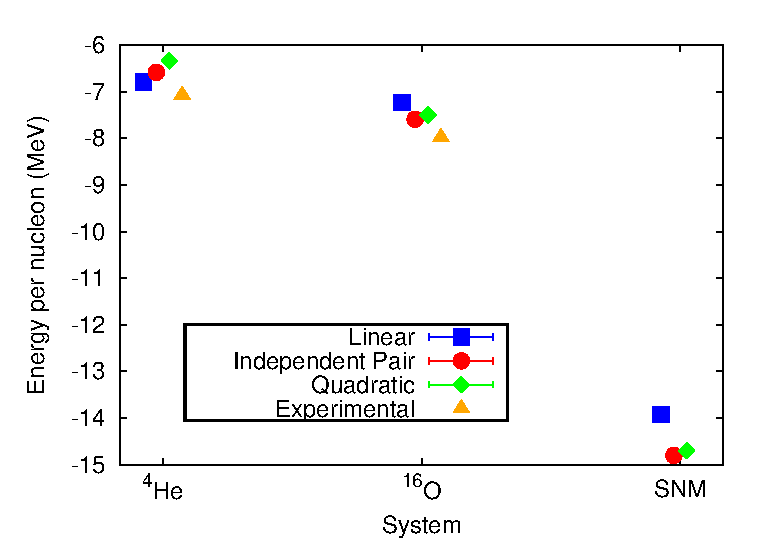
\includegraphics[width=0.5\textwidth]{energy.eps}
   \caption{Energy per nucleon for ${}^4$He and ${}^{16}$O as calculated with linear, independent pair and quadratic correlations. Also, the energy per nucleon of symmetric nuclear matter of 28 particles in a periodic box with density $\rho=0.16$fm$^{-3}$. All calculations are compared to their expected values.}
   \label{fig:energies}
\end{figure}
Notice that in the case of ${}^{16}$O and SNM the independent pair and quadratic correlations caused the energies to decrease, while in the case of ${}^4$He the energy went up when independent pair correlations were added, and even more when the quadratic correlations were added. We expected the energies and uncertainties to decrease a little for each calculation since we were using a more correct wave function. This was true for $^{16}$O and SNM, but not for $^{4}$He. The energy for $^{4}$He increased with both new types of correlations. At first we thought that this could be due to the small number of extra terms in the independent pair correlation with only 4 particles, however the quadratic correlations, which have many more terms, also caused the energy to increase. %%To determine if this increase was reasonable we did calculations for $^{4}$He with all three correlations with the constraint removed. The constraint is used to control the fermion-sign problem and when unconstrained calculations are controlled they should converge to the exact answer. We did calculations to see if all three correlation types would converge to the same value. There was evidence that this was the case, but the data became too noisy to be sure. 
The original linearly correlated wave function had been well optimized, but the  quadratic correlations were included without any additional optimization. We included a simple optimization factor in the front of the independent pair correlations for $^4$He and it is clear that additional optimization is needed to minimize the energy as can be seen in figure~\ref{fig:quadfact}.
\begin{figure}[h!]
   \centering
   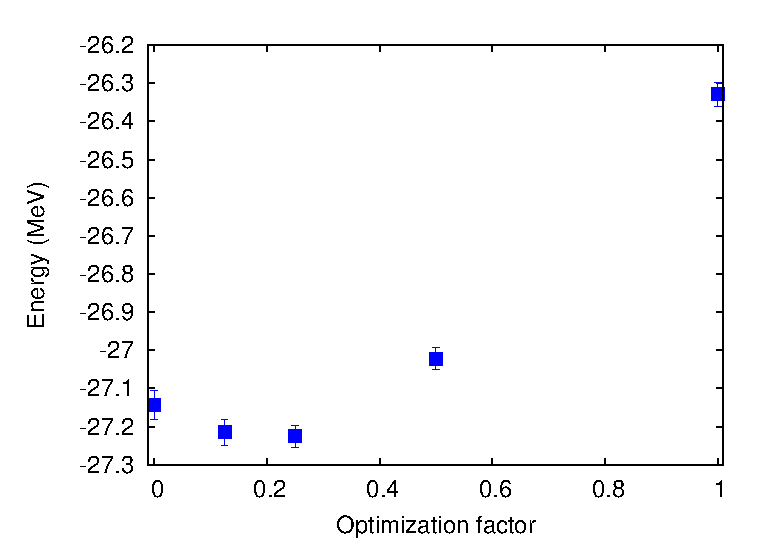
\includegraphics[width=0.5\textwidth]{quadfact.eps}
   \caption{Energy for $^4$He as a function of the quadratic correlation optimization parameter, calculated with independent pair correlations.}
   \label{fig:quadfact}
\end{figure}
The scaling of the calculations with independent pair and quadratic correlations in relation to the original linear correlations is given in Fig.~\ref{fig:scaling}. The scaling factors were calculated by comparing the average times it took to complete one block of calculations to the average times it took for the linear correlations.



To calculate the scaling the average time to complete one block of calculations was used.
\begin{figure}[h!]
   \centering
   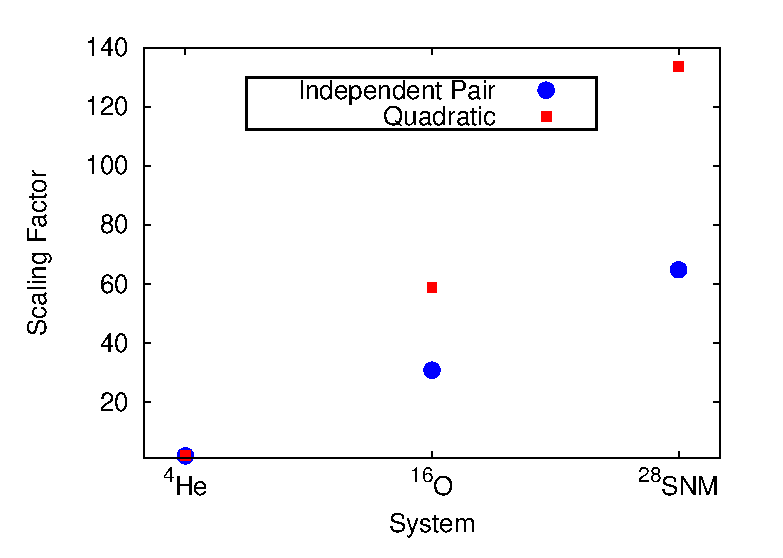
\includegraphics[width=0.5\textwidth]{scaling.eps}
   \caption{Scaling factors for ${}^4$He, ${}^{16}$O, and symmetric nuclear matter as calculated with the average time to complete a block of calculations. The factor is a ratio of the time to calculate the independent pair calculations compared to the time to calculate with the linear correlations. The factors are 1.73, 30.74 and 64.77 respectively for independent pair correlations, and 2.00, 58.83 and 133.59 for quadratic correlations..}
   \label{fig:scaling}
\end{figure}
